A dashboard is a page laid out with multiple charts, plots, and
visualizations all together. You define the layout with a YAML
configuration file which contains the types of plots and their
configurations all in one place.

\begin{figure}[H]
  \centering
  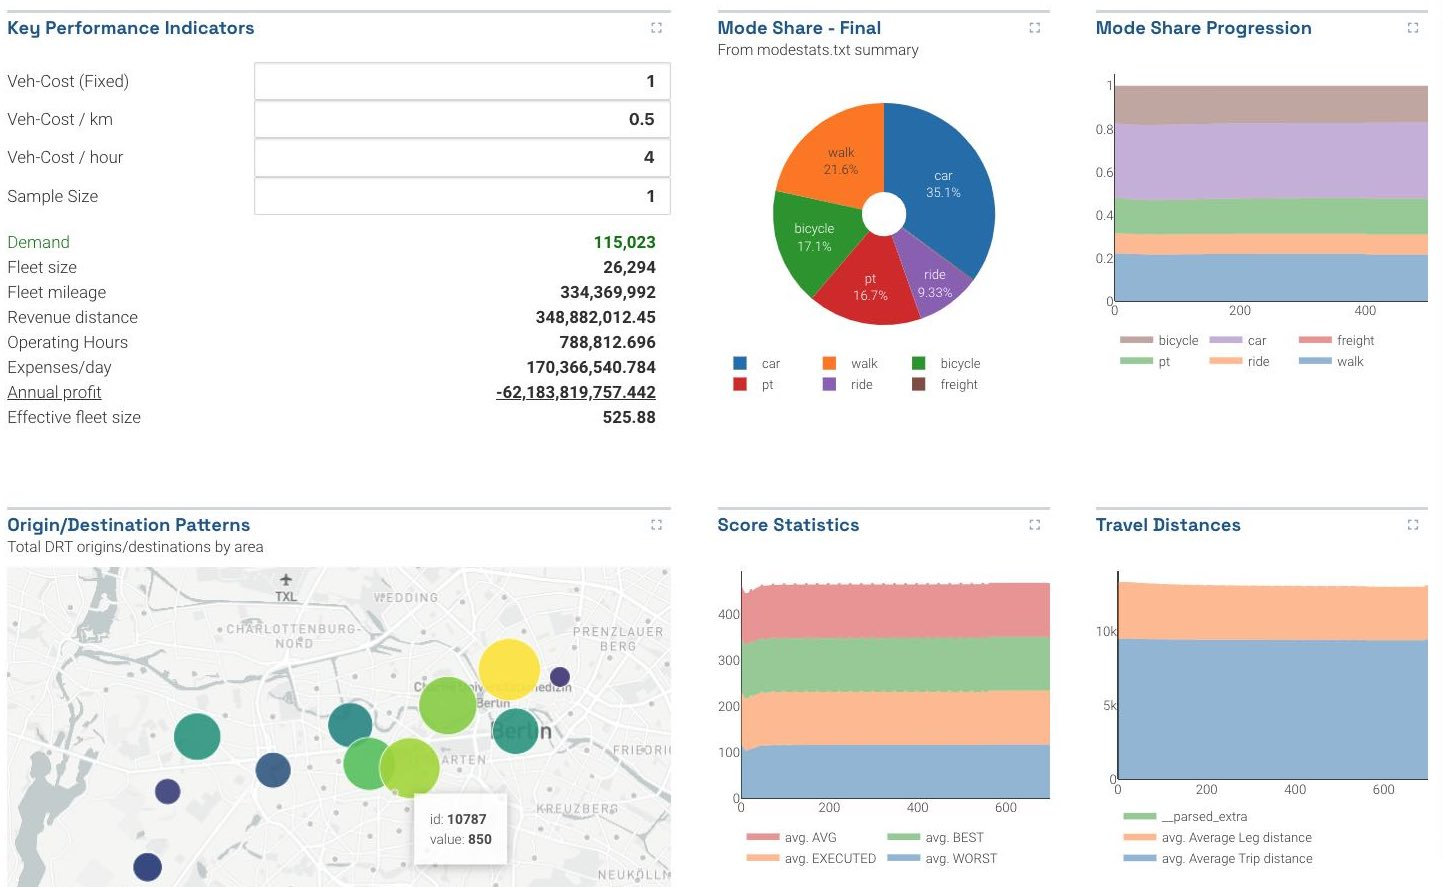
\includegraphics[width=0.8\textwidth]{assets/dashboard.jpg}
  \caption{Dashboards usually show several at-a-glance summary metrics.}
\end{figure}

A folder containing any number of \texttt{dashboard-*} YAML files show
the dashboard instead of the usual folder browser view. When multiple
dashboard YAML files exist, they will be shown as multiple navigation
tabs on the page.

\hypertarget{defining-a-dashboard}{%
\subsection{Defining a dashboard}\label{defining-a-dashboard}}

Start with the example below and edit as necessary. YAML is
\emph{extremely picky} about white space and indentation, like Python.
Be careful!

\hypertarget{header}{%
\subsubsection{Header}\label{header}}

A dashboard requires a top-level \texttt{header} containing \emph{tab}
and \emph{title} and optional \emph{description.}

\begin{lstlisting}
  header:
  tab: 'Summary'
  title: 'Top-Level Summary Statistics'
  description: 'At-a-glance figures we usually look at' #optional
\end{lstlisting}

\hypertarget{layout}{%
\subsubsection{Layout}\label{layout}}

Below the header, a dashboard also requires a \texttt{layout} section
which defines a set of named \textbf{rows}. The row name themselves are
not displayed anywhere; they are just there to help you organize the
file.

\textbf{row}: Each \texttt{row} can contain either (1) the properties of
a full-width panel, or (2) a YAML \textbf{list} of properties for panels
that will be laid out horizontally in the row. YAML lists have a strange
syntax with \texttt{-} hyphens marking the beginning of a list item.
It's best to just look at the example below.

By default, multiple panels are laid out from left to right, in equal widths. (But see \emph{width} option further below)

\begin{lstlisting}
  layout:
  myRow1: # this row has one full-width chart
    type: bar
    title: 'My Bar Chart'
    dataset: mycsvdata.csv
    # ...

  # next row has two charts, using the '-' YAML list syntax
  myMultiRow:
    - type: bar
      title: 'My Bar Chart'
      dataset: mycsvdata.csv
      # ...

    - type: table
      title: 'My Summary Table'
      config: summary-table.yaml
\end{lstlisting}

That indentation in the example above is extremely important!
Indentation is how YAML interprets the grouping of elements.

\textbf{Chart/plot details:} Each element in a row has the following
properties. This defines the actual chart that will be displayed.

\begin{itemize}
\tightlist
\item
  \textbf{type} Required: the chart or plot type, e.g.~\texttt{pie},
  \texttt{bar}, \texttt{flowmap}, etc. See the individual chart docs for
  all available plots.
\item
  \textbf{title} The name of the plot
\item
  \textbf{description} A brief description (optional)
\item
  \textbf{height} You can set \emph{relative height} by adding the
  \texttt{height:} parameter (default: 5)
\item
  \textbf{width} You can set \emph{relative widths} by adding the
  \texttt{width:\ {[}number{]}} property. Panels have a default width of
  1. Thus in a row with 3 charts, if the width of the first object is 2,
  then {[}2+1+1{]} means the first object fills 50\% of the row, and the
  remaining two objects fill 25\% each. (default: 1)
\item
  \textbf{Other properties} Every viz type has its own set of
  properties. Include those as separate \texttt{key:\ value} lines in
  the configuration, as needed. See the individual chart docs in the API
  Reference; \emph{The chart type determines the set of valid
  properties!}
\end{itemize}

\hypertarget{example-dashboard-summary.yaml}{%
\subsection{Example:
dashboard-summary.yaml}\label{example-dashboard-summary.yaml}}

Here is a full example dashboard, pulling all of the above together.
Note especially the indentation and the use of \texttt{-} to denote YAML
lists.

\begin{lstlisting}
header:
  tab: Summary
  title: My Summary Dashboard
  description: 'Examples of various chart types'

layout:
  row1: # this row has two charts
    - title: 'Mode Share - Final'
      description: 'From modestats.txt summary'
      type: 'pie'
      width: 1
      dataset: '*modestats.txt'
      useLastRow: true
      ignoreColumns: ['Iteration']

    - title: 'Example Bar Plot'
      description: 'Distance over Iteration'
      type: 'bar'
      width: 2
      usedCol: [distance_m_mean, directDistance_m_mean]
      legendName: [Distance (mean), Direct Distance (mean)]
      skipFirstRow: true
      dataset: '*drt_customer_stats_drt_short.csv'
      x: 'iteration'
      yAxisName: 'Distanz'
      xAxisName: 'Iteration'

  secondRow: # this row has just one plot
    title: 'Example Line Plot'
    description: 'Distance over Iteration'
    type: 'line'
    width: 1
    usedCol: [distance_m_mean, directDistance_m_mean]
    legendName: [Distance (mean), Direct Distance (mean)]
    skipFirstRow: false
    dataset: '*drt_customer_stats_drt.csv'
    x: 'iteration'
    yAxisName: 'Distance'
    xAxisName: 'Iteration'
\end{lstlisting}